\documentclass[11pt,letterpaper]{article}
\usepackage[lmargin=1in,rmargin=1in,tmargin=1in,bmargin=1in]{geometry}
\usepackage{../style/homework}
\usepackage{../style/commands}
\setbool{quotetype}{false} % True: Side; False: Under
\setbool{hideans}{true} % Student: True; Instructor: False

% -------------------
% Content
% -------------------
\begin{document}

\homework{15: Due 05/01}{True optimization is the revolutionary contribution of modern research to decision processes.}{George Dantzig}

% Problem 1
\problem{10} Find the maximum and minimum values for the function $z= 4x_1 + 5x_2$ on the region shown below. Be sure to fully justify that your answers are correct. 
	\[
	\fbox{
	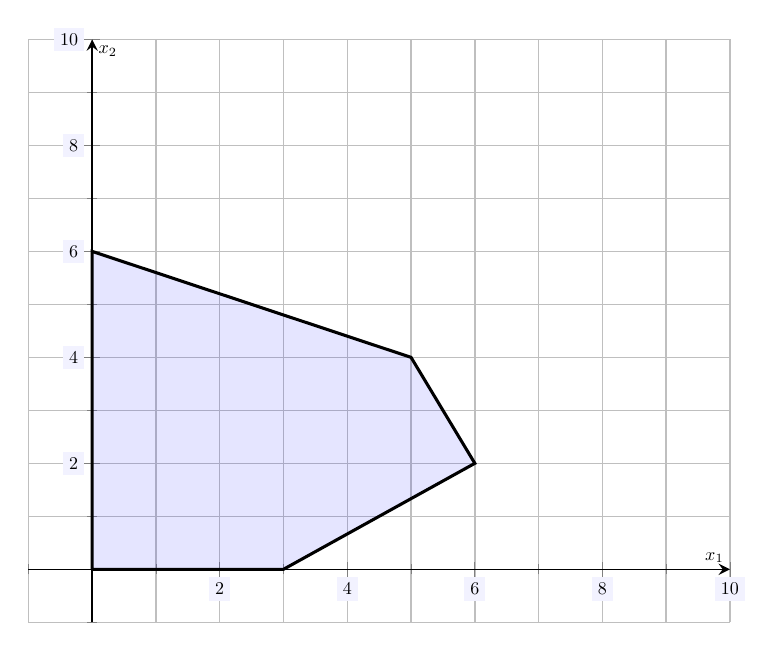
\begin{tikzpicture}[scale=1.3,every node/.style={scale=0.5}]
	\begin{axis}[
	grid=both,
	axis lines=middle,
	ticklabel style={fill=blue!5!white},
	xmin= -1, xmax=10,
	ymin= -1, ymax=10,
	xtick={0,2,4,6,8,10},
	ytick={0,2,4,6,8,10},
	minor tick = {-1,0,1,...,10},
	xlabel=\(x_1\),ylabel=\(x_2\),
	]
%	\addplot[domain= -1:10, line width=0.03cm] (x,5-x);
%	\draw[line width=0.03cm] (3,-10.5) -- (3,10.5);
	\draw[line width=0.01cm,fill= blue,opacity=0.1] (0,0) -- (0,6) -- (5,4) -- (6,2) -- (3,0) -- (0,0);
	\draw[line width=0.03cm] (0,0) -- (0,6) -- (5,4) -- (6,2) -- (3,0) -- (0,0);
	\end{axis}
	\end{tikzpicture}
	}
	\]



\newpage



% Problem 2
\problem{10} Consider the function $z= 5x_1 - x_2$. Does this function has a maximum on the region shown below? If so, explain and find the maximum. If not, explain why. Answer the same question for the minimum of $z$ on the region shown below. 
	\[
	\fbox{
	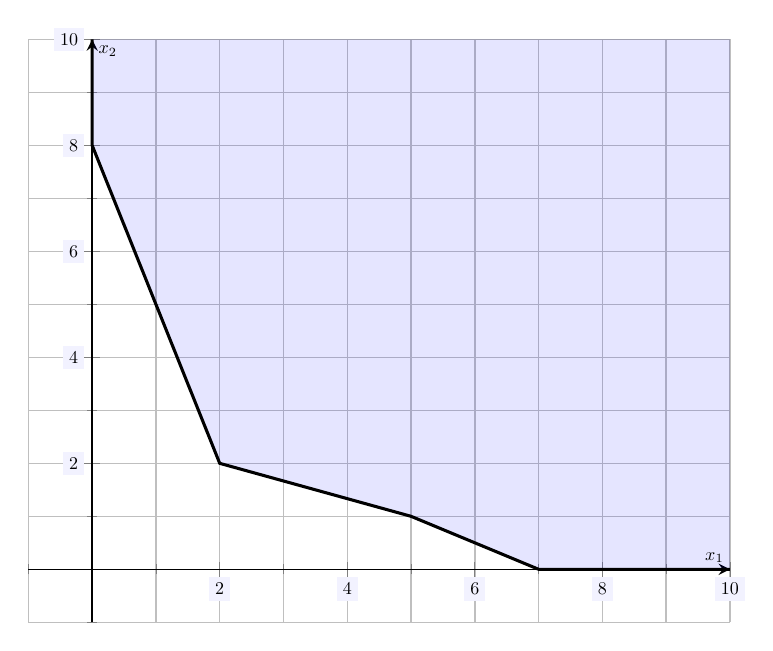
\begin{tikzpicture}[scale=1.3,every node/.style={scale=0.5}]
	\begin{axis}[
	grid=both,
	axis lines=middle,
	ticklabel style={fill=blue!5!white},
	xmin= -1, xmax=10,
	ymin= -1, ymax=10,
	xtick={0,2,4,6,8,10},
	ytick={0,2,4,6,8,10},
	minor tick = {-1,0,1,...,10},
	xlabel=\(x_1\),ylabel=\(x_2\),
	]
%	\addplot[domain= -1:10, line width=0.03cm] (x,5-x);
%	\draw[line width=0.03cm] (3,-10.5) -- (3,10.5);
	\draw[line width=0.01cm,fill= blue,opacity=0.1] (0,8) -- (0,10) -- (10,10) -- (10,0) -- (7,0) -- (5,1) -- (2,2) -- (0,8);
	\draw[line width=0.03cm] (0,10) -- (0,8) -- (2,2) -- (5,1) -- (7,0) -- (10,0);
	\end{axis}
	\end{tikzpicture}
	}
	\]























\end{document}